\documentclass[aspectratio=169]{beamer}
\usepackage{booktabs}
\usepackage{pgfplots}
\pgfplotsset{compat=1.18}
\usepackage{tikz}
\usetikzlibrary{shapes.geometric,arrows.meta,positioning,fit,backgrounds,calc,decorations.pathreplacing}
\usepackage{xcolor}
\usepackage{colortbl}
\usepackage{multirow}
\usepackage{array}
\usepackage{amsmath}

\definecolor{NXPOrange}{RGB}{255,102,0}
\definecolor{NXPBlue}{RGB}{0,56,101}
\definecolor{NXPGreen}{RGB}{0,153,76}
\definecolor{NXPGray}{RGB}{100,100,100}
\definecolor{LightOrange}{RGB}{255,240,220}
\definecolor{LightBlue}{RGB}{220,235,255}
\definecolor{AccentRed}{RGB}{200,0,50}
\definecolor{DarkGray}{RGB}{50,50,50}

\usetheme{Madrid}
\usecolortheme[named=NXPBlue]{structure}
\setbeamercolor{title}{fg=white,bg=NXPBlue}
\setbeamercolor{frametitle}{fg=white,bg=NXPBlue}
\setbeamercolor{block title}{fg=white,bg=NXPBlue}
\setbeamercolor{block title alerted}{fg=white,bg=NXPOrange}
\setbeamerfont{title}{size=\Large,series=\bfseries}
\setbeamerfont{frametitle}{size=\normalsize,series=\bfseries}
\setbeamertemplate{navigation symbols}{}
\setbeamertemplate{footline}[frame number]

\title{NXP eIQ}
\subtitle{Hardware Products \& Model Zoo Fit Analysis}
\author{Edge AI Platform Evaluation}
\date{August 2026}
\institute{NXP Semiconductors}

\begin{document}

\begin{frame}\titlepage\end{frame}
\begin{frame}{Agenda}\tableofcontents\end{frame}

\section{NXP Edge AI Product Portfolio}

\begin{frame}{NXP Edge AI Platform Spectrum}
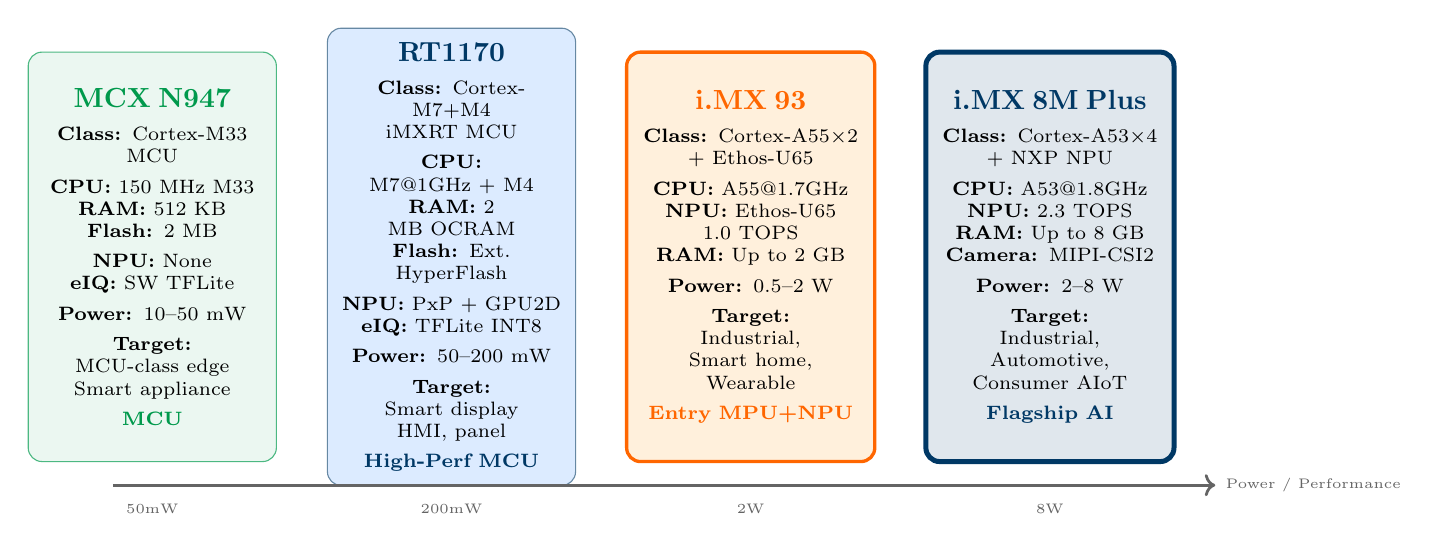
\begin{tikzpicture}[
  dev/.style={rounded corners=5pt,minimum width=3.0cm,
              minimum height=5.2cm,text width=2.8cm,align=center,
              font=\scriptsize,inner sep=5pt},
]
% MCX N947 --- MCU entry
\node[dev,draw=NXPGreen!70,fill=NXPGreen!8] (mcx) at (0,0) {
  \textcolor{NXPGreen}{\textbf{\normalsize MCX N947}}\\[4pt]
  \textbf{Class:} Cortex-M33\\MCU\\[3pt]
  \textbf{CPU:} 150 MHz M33\\
  \textbf{RAM:} 512 KB\\
  \textbf{Flash:} 2 MB\\[3pt]
  \textbf{NPU:} None\\
  \textbf{eIQ:} SW TFLite\\[3pt]
  \textbf{Power:} 10--50 mW\\[3pt]
  \textbf{Target:}\\MCU-class edge\\Smart appliance\\[3pt]
  \textcolor{NXPGreen}{\textbf{MCU}}
};
% RT1170 --- MCU with NPU
\node[dev,draw=NXPBlue!60,fill=LightBlue] (rt) at (3.8,0) {
  \textcolor{NXPBlue}{\textbf{\normalsize RT1170}}\\[4pt]
  \textbf{Class:} Cortex-M7+M4\\iMXRT MCU\\[3pt]
  \textbf{CPU:} M7@1GHz + M4\\
  \textbf{RAM:} 2 MB OCRAM\\
  \textbf{Flash:} Ext. HyperFlash\\[3pt]
  \textbf{NPU:} PxP + GPU2D\\
  \textbf{eIQ:} TFLite INT8\\[3pt]
  \textbf{Power:} 50--200 mW\\[3pt]
  \textbf{Target:}\\Smart display\\HMI, panel\\[3pt]
  \textcolor{NXPBlue}{\textbf{High-Perf MCU}}
};
% i.MX 93 --- entry MPU + Ethos
\node[dev,draw=NXPOrange,fill=LightOrange,line width=1.2pt] (imx93) at (7.6,0) {
  \textcolor{NXPOrange}{\textbf{\normalsize i.MX 93}}\\[4pt]
  \textbf{Class:} Cortex-A55$\times$2\\+ Ethos-U65\\[3pt]
  \textbf{CPU:} A55@1.7GHz\\
  \textbf{NPU:} Ethos-U65\\1.0 TOPS\\
  \textbf{RAM:} Up to 2 GB\\[3pt]
  \textbf{Power:} 0.5--2 W\\[3pt]
  \textbf{Target:}\\Industrial,\\Smart home,\\Wearable\\[3pt]
  \textcolor{NXPOrange}{\textbf{Entry MPU+NPU}}
};
% i.MX 8M Plus --- flagship
\node[dev,draw=NXPBlue,fill=NXPBlue!12,line width=1.8pt] (imx8) at (11.4,0) {
  \textcolor{NXPBlue}{\textbf{\normalsize i.MX 8M Plus}}\\[4pt]
  \textbf{Class:} Cortex-A53$\times$4\\+ NXP NPU\\[3pt]
  \textbf{CPU:} A53@1.8GHz\\
  \textbf{NPU:} 2.3 TOPS\\
  \textbf{RAM:} Up to 8 GB\\
  \textbf{Camera:} MIPI-CSI2\\[3pt]
  \textbf{Power:} 2--8 W\\[3pt]
  \textbf{Target:}\\Industrial,\\Automotive,\\Consumer AIoT\\[3pt]
  \textcolor{NXPBlue}{\textbf{Flagship AI}}
};
% Power axis
\draw[->,NXPGray,line width=1pt] (-0.5,-2.9) -- (13.5,-2.9)
  node[right,font=\tiny,text=NXPGray]{Power / Performance};
\foreach \x/\lbl in {0/50mW,3.8/200mW,7.6/2W,11.4/8W}
  \node[font=\tiny,text=NXPGray] at (\x,-3.2) {\lbl};
\end{tikzpicture}
\end{frame}

\begin{frame}{NXP Edge AI Device Specifications}
\small
\begin{tabular}{lcccc}
\toprule
\textbf{Spec} & \textbf{MCX N947} & \textbf{RT1170} & \textbf{i.MX 93} & \textbf{i.MX 8M Plus}\\
\midrule
\textbf{Primary CPU} & M33 150MHz & M7 1GHz+M4 & A55$\times$2 1.7GHz & A53$\times$4 1.8GHz\\
\textbf{NPU} & None & PxP (limited) & Ethos-U65 & NXP NPU 2.3T\\
\textbf{NPU TOPS} & --- & $<$0.1 & 1.0 & 2.3\\
\textbf{RAM} & 512 KB & 2 MB OCRAM & 2 GB LPDDR4 & 8 GB LPDDR4\\
\textbf{Power (TDP)} & 10--50 mW & 50--200 mW & 0.5--2 W & 2--8 W\\
\textbf{OS} & RTOS (Zephyr) & FreeRTOS & Linux / Zephyr & Linux (Yocto)\\
\textbf{eIQ stack} & TFLite Micro & TFLite & TFLite+Vela & TFLite+PyTorch\\
\textbf{Model format} & TFLite INT8 & TFLite INT8 & .tflite+.tosa & .tflite\\
\textbf{Vela support} & No & No & \textbf{Yes} & No\\
\textbf{Video input} & --- & MIPI-DSI & MIPI-CSI & 2$\times$ MIPI-CSI\\
\textbf{Process node} & 40 nm & 28 nm & 16 nm & 14 nm\\
\textbf{Model zoo models} & 6 & 8 & 9 & 18\\
\bottomrule
\end{tabular}
\end{frame}

\begin{frame}{i.MX 8M Plus NPU: 2.3 TOPS Architecture}
\begin{columns}
\column{0.52\textwidth}
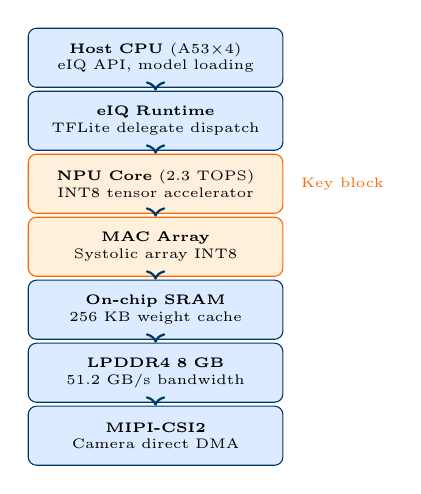
\begin{tikzpicture}[
  blk/.style={draw=NXPBlue,fill=LightBlue,rounded corners=3pt,
              minimum height=0.75cm,text width=3.0cm,align=center,font=\tiny},
  ablk/.style={draw=NXPOrange,fill=LightOrange,rounded corners=3pt,
               minimum height=0.75cm,text width=3.0cm,align=center,font=\tiny},
]
\node[blk] (cpu) at (0,5.0) {\textbf{Host CPU} (A53$\times$4)\\eIQ API, model loading};
\node[blk] (eiq) at (0,4.2) {\textbf{eIQ Runtime}\\TFLite delegate dispatch};
\node[ablk] (npu) at (0,3.4) {\textbf{NPU Core} (2.3 TOPS)\\INT8 tensor accelerator};
\node[ablk] (mac) at (0,2.6) {\textbf{MAC Array}\\Systolic array INT8};
\node[blk] (sram) at (0,1.8) {\textbf{On-chip SRAM}\\256 KB weight cache};
\node[blk] (lpddr) at (0,1.0) {\textbf{LPDDR4 8 GB}\\51.2 GB/s bandwidth};
\node[blk] (csi) at (0,0.2) {\textbf{MIPI-CSI2}\\Camera direct DMA};
\foreach \a/\b in {cpu/eiq,eiq/npu,npu/mac,mac/sram,sram/lpddr,lpddr/csi}
  \draw[->,NXPBlue,line width=0.8pt] (\a) -- (\b);
\node[right=0.1cm of npu,font=\tiny,text=NXPOrange] {Key block};
\end{tikzpicture}
\column{0.45\textwidth}
\footnotesize
\begin{block}{NPU Features}
\begin{itemize}
  \item \textbf{2.3 TOPS} peak (INT8)
  \item Supports: Conv2D, DW-Conv, BN, ReLU, Pooling, FC, Sigmoid, LSTM
  \item \textbf{Per-channel quantization}: better accuracy than per-tensor
  \item \textbf{TFLite delegate}: seamless fallback to CPU for unsupported ops
  \item LPDDR4 BW: 51.2 GB/s sustains large models
\end{itemize}
\end{block}
\begin{alertblock}{Ethos-U65 (i.MX 93)}
\footnotesize Arm Ethos-U65 microNPU on i.MX 93: 1.0 TOPS, requires \textbf{Vela compiler} to convert TFLite $\rightarrow$ optimized Ethos command stream.
\end{alertblock}
\end{columns}
\end{frame}

\section{eIQ Software Stack}

\begin{frame}{NXP eIQ Software Stack: recipe.sh Flow}
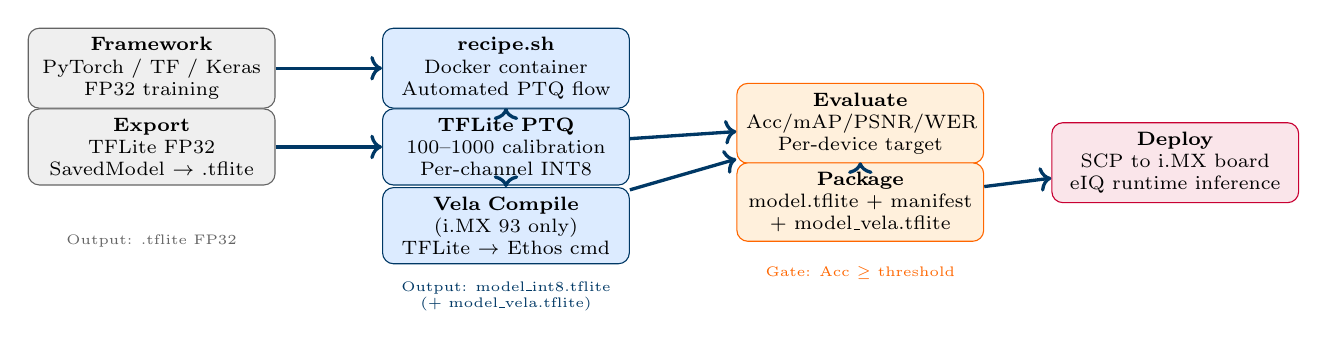
\begin{tikzpicture}[
  box/.style={rounded corners=4pt,minimum height=0.85cm,
              text width=2.9cm,align=center,font=\scriptsize},
  arr/.style={->,line width=1.2pt,NXPBlue},
]
\node[draw=NXPGray,fill=NXPGray!10,box] (fw) at (0,3.2)
  {\textbf{Framework}\\PyTorch / TF / Keras\\FP32 training};
\node[draw=NXPGray,fill=NXPGray!10,box] (exp) at (0,2.2)
  {\textbf{Export}\\TFLite FP32\\SavedModel $\rightarrow$ .tflite};
\node[draw=NXPBlue,fill=LightBlue,box] (recipe) at (4.5,3.2)
  {\textbf{recipe.sh}\\Docker container\\Automated PTQ flow};
\node[draw=NXPBlue,fill=LightBlue,box] (ptq) at (4.5,2.2)
  {\textbf{TFLite PTQ}\\100--1000 calibration\\Per-channel INT8};
\node[draw=NXPBlue,fill=LightBlue,box] (vela) at (4.5,1.2)
  {\textbf{Vela Compile}\\(i.MX 93 only)\\TFLite $\rightarrow$ Ethos cmd};
\node[draw=NXPOrange,fill=LightOrange,box] (eval) at (9.0,2.5)
  {\textbf{Evaluate}\\Acc/mAP/PSNR/WER\\Per-device target};
\node[draw=NXPOrange,fill=LightOrange,box] (pkg) at (9.0,1.5)
  {\textbf{Package}\\model.tflite + manifest\\+ model\_vela.tflite};
\node[draw=AccentRed,fill=AccentRed!10,box] (deploy) at (13.0,2.0)
  {\textbf{Deploy}\\SCP to i.MX board\\eIQ runtime inference};
\draw[arr] (fw) -- (recipe);
\draw[arr] (exp) -- (ptq);
\draw[arr] (recipe) -- (ptq);
\draw[arr] (ptq) -- (vela);
\draw[arr] (ptq) -- (eval);
\draw[arr] (vela) -- (eval);
\draw[arr] (eval) -- (pkg);
\draw[arr] (pkg) -- (deploy);
\node[font=\tiny,text=NXPGray,align=center] at (0,1.0)
  {Output: .tflite FP32};
\node[font=\tiny,text=NXPBlue,align=center] at (4.5,0.3)
  {Output: model\_int8.tflite\\(+ model\_vela.tflite)};
\node[font=\tiny,text=NXPOrange,align=center] at (9.0,0.6)
  {Gate: Acc $\geq$ threshold};
\end{tikzpicture}
\end{frame}

\begin{frame}{Vela Compiler: TFLite $\rightarrow$ Ethos-U65 Optimization}
\begin{columns}
\column{0.55\textwidth}
\begin{tikzpicture}[
  step/.style={draw=NXPOrange,fill=LightOrange,rounded corners=3pt,
               minimum height=0.75cm,text width=3.8cm,align=left,
               font=\tiny,inner sep=4pt},
]
\node[step] (s1) at (0,4.0) {\textbf{Input}: model\_int8.tflite\\Standard TFLite INT8 model};
\node[step] (s2) at (0,3.2) {\textbf{Op partition}: supported ops $\rightarrow$ Ethos\\unsupported ops $\rightarrow$ Cortex-A55};
\node[step] (s3) at (0,2.4) {\textbf{Memory planning}: SRAM tiling\\Minimise DRAM bandwidth};
\node[step] (s4) at (0,1.6) {\textbf{Operator scheduling}: pipeline\\overlaps DMA + compute};
\node[step] (s5) at (0,0.8) {\textbf{Output}: model\_vela.tflite\\Ethos-U65 command stream};
\node[step] (s6) at (0,0.0) {\textbf{Speedup}: 2--4$\times$ vs CPU TFLite\\on i.MX 93 Ethos-U65};
\foreach \a/\b in {s1/s2,s2/s3,s3/s4,s4/s5,s5/s6}
  \draw[->,NXPOrange,line width=0.8pt] (\a) -- (\b);
\end{tikzpicture}
\column{0.42\textwidth}
\footnotesize
\begin{block}{Ethos-U65 Supported Ops}
\begin{itemize}
  \item Conv2D, DepthwiseConv2D
  \item MaxPool, AvgPool, GlobalAvgPool
  \item FC (Dense), Sigmoid, ReLU/ReLU6
  \item Concatenate, Reshape, Transpose
  \item BatchMatMul (limited)
\end{itemize}
\end{block}
\begin{block}{Typical Speedups on i.MX 93}
\footnotesize
\begin{tabular}{@{}lcc@{}}
\textbf{Model} & \textbf{CPU} & \textbf{Ethos-U65}\\
\midrule
MobileNetV2 & 120ms & 30ms\\
NanoDet-M & 480ms & 115ms\\
DS-CNN & 15ms & 4ms\\
\end{tabular}
\end{block}
\end{columns}
\end{frame}

\section{Model Zoo: Classification}

\begin{frame}{Classification Models --- Hardware Fit Matrix}
\small
\begin{tabular}{lccccl}
\toprule
\textbf{Model} & \textbf{Top-1} & \textbf{Params} & \textbf{MCX/RT} & \textbf{i.MX 93} & \textbf{i.MX 8M+}\\
\midrule
mobilenetv1\_025 & 50.2\% & 0.5M & \textcolor{NXPGreen}{\checkmark\checkmark} & \checkmark & \checkmark\\
mobilenetv1 & 70.9\% & 4.2M & \textcolor{NXPGreen}{\checkmark\checkmark} & \checkmark & \checkmark\\
mobilenetv2 & 71.8\% & 3.4M & \textcolor{NXPGreen}{\checkmark\checkmark} & \checkmark & \checkmark\\
mnasnet & 72.3\% & 4.0M & \textcolor{NXPGreen}{\checkmark\checkmark} & \checkmark & \checkmark\\
efficientnet\_lite0 & 72.2\% & 5.6M & $\circ$ & \textcolor{NXPGreen}{\checkmark\checkmark} & \checkmark\\
efficientnet\_lite2 & 75.1\% & 6.9M & $\circ$ & \textcolor{NXPGreen}{\checkmark\checkmark} & \checkmark\\
resnet50 & 75.9\% & 25M & $\times$ & $\circ$ & \textcolor{NXPGreen}{\checkmark\checkmark}\\
inceptionv4 & 78.2\% & 43M & $\times$ & $\times$ & \textcolor{NXPGreen}{\checkmark\checkmark}\\
mobilenetv3\_large & 73.0\% & 5.5M & $\circ$ & \textcolor{NXPGreen}{\checkmark\checkmark} & \checkmark\\
\midrule
\multicolumn{6}{l}{\footnotesize \textcolor{NXPGreen}{\checkmark\checkmark} = optimal \quad \checkmark = supported \quad $\circ$ = borderline \quad $\times$ = not recommended}
\end{tabular}
\end{frame}

\begin{frame}{Classification Accuracy vs.\ Target Platform}
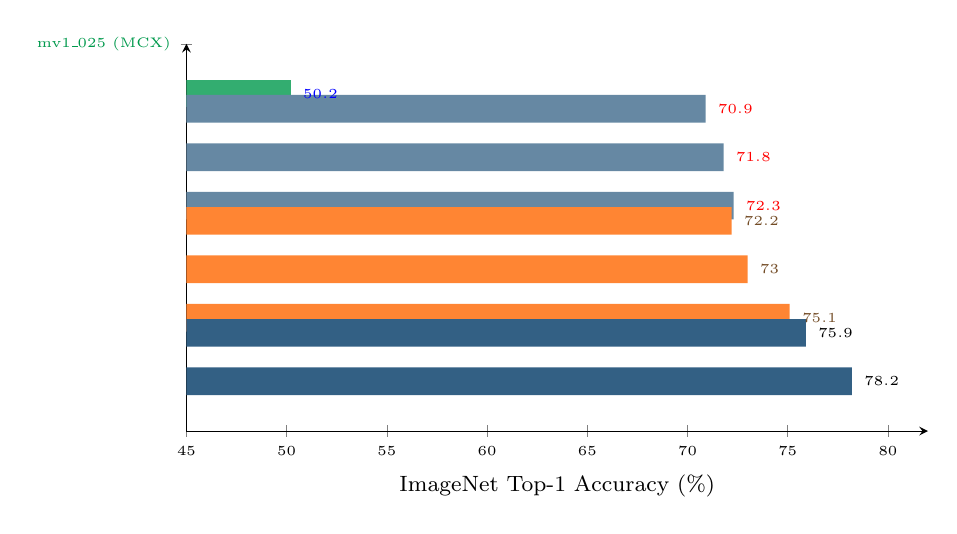
\begin{tikzpicture}
\begin{axis}[
  xbar,
  width=11cm, height=6.5cm,
  bar width=10pt,
  xlabel={\footnotesize ImageNet Top-1 Accuracy (\%)},
  ytick=data,
  yticklabels={
    \textcolor{NXPGreen}{mv1\_025 (MCX)},
    \textcolor{NXPBlue}{mobilenetv1 (RT1170)},
    \textcolor{NXPBlue}{mobilenetv2 (RT1170)},
    \textcolor{NXPBlue}{mnasnet (RT1170)},
    \textcolor{NXPOrange}{efficientnet\_lite0 (i93)},
    \textcolor{NXPOrange}{mobilenetv3\_large (i93)},
    \textcolor{NXPOrange}{efficientnet\_lite2 (i93)},
    \textcolor{NXPBlue}{resnet50 (8M+)},
    \textcolor{NXPBlue}{inceptionv4 (8M+)}
  },
  yticklabel style={font=\tiny},
  xticklabel style={font=\tiny},
  xmin=45,xmax=82,
  tick align=inside,axis lines=left,
  nodes near coords,nodes near coords style={font=\tiny,xshift=1pt},
]
\addplot+[xbar,fill=NXPGreen!80,draw=none] coordinates {(50.2,8)};
\addplot+[xbar,fill=NXPBlue!60,draw=none]
  coordinates {(70.9,7)(71.8,6)(72.3,5)};
\addplot+[xbar,fill=NXPOrange!80,draw=none]
  coordinates {(72.2,4)(73.0,3)(75.1,2)};
\addplot+[xbar,fill=NXPBlue!80,draw=none]
  coordinates {(75.9,1)(78.2,0)};
\end{axis}
\end{tikzpicture}
\end{frame}

\section{Model Zoo: Detection \& Segmentation}

\begin{frame}{Detection Models --- Platform Fit}
\small
\begin{tabular}{lcccl}
\toprule
\textbf{Model} & \textbf{mAP} & \textbf{Target} & \textbf{Latency} & \textbf{Why fits}\\
\midrule
nanodet\_m & 23.5\% & i.MX 93 & 115ms (Ethos) & Tiny: 1.8M, Vela optimised\\
ssdlite\_mv2 & 31.8\% & RT1170 & $\sim$80ms & SSD anchor-based, TFLite std\\
ssdlite\_mv3 & 34.2\% & RT1170 & $\sim$90ms & MNv3 backbone, RT1170 2MB\\
efficientdet\_lite0 & 33.0\% & i.MX 93 & $\sim$120ms & BiFPN light, Ethos-friendly\\
efficientdet\_lite2 & 37.5\% & i.MX 8M Plus & $\sim$60ms & Needs 2.3 TOPS NPU\\
yolov5s & 40.0\% & i.MX 8M Plus & $\sim$50ms & Full CSP backbone\\
yolov8m & 53.5\% & i.MX 8M Plus & $\sim$75ms & Best det mAP in zoo\\
\midrule
\multicolumn{5}{l}{\textit{Segmentation}}\\
deeplabv3 & 58.0\% & i.MX 8M Plus & $\sim$80ms & ASPP: needs 2.3 TOPS\\
fcn\_mobilenetv2 & 52.0\% & i.MX 93 & $\sim$100ms & Lighter FCN head, Vela ok\\
\bottomrule
\end{tabular}
\end{frame}

\section{NXP-Exclusive: SR, Face \& BCI}

\begin{frame}{NXP-Exclusive Models: SR + Face Recognition + BCI}
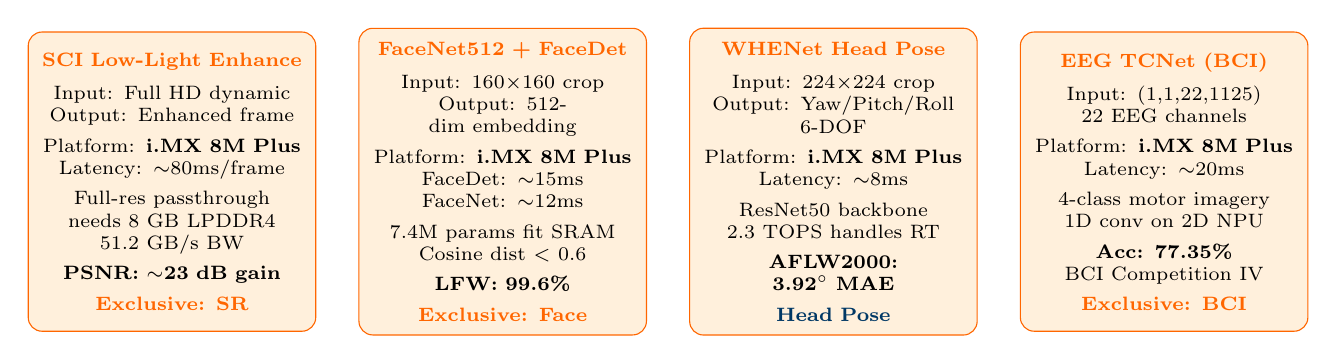
\begin{tikzpicture}[
  modblk/.style={draw=NXPOrange,fill=LightOrange,rounded corners=5pt,
                 minimum height=3.8cm,text width=3.3cm,align=center,
                 font=\scriptsize,inner sep=5pt},
]
\node[modblk] (sci) at (0,0) {
  \textcolor{NXPOrange}{\textbf{SCI Low-Light Enhance}}\\[4pt]
  Input: Full HD dynamic\\
  Output: Enhanced frame\\[3pt]
  Platform: \textbf{i.MX 8M Plus}\\
  Latency: $\sim$80ms/frame\\[3pt]
  Full-res passthrough\\needs 8 GB LPDDR4\\51.2 GB/s BW\\[3pt]
  \textbf{PSNR: $\sim$23 dB gain}\\[3pt]
  \textcolor{NXPOrange}{\textbf{Exclusive: SR}}
};
\node[modblk] (fn) at (4.2,0) {
  \textcolor{NXPOrange}{\textbf{FaceNet512 + FaceDet}}\\[4pt]
  Input: 160$\times$160 crop\\
  Output: 512-dim embedding\\[3pt]
  Platform: \textbf{i.MX 8M Plus}\\
  FaceDet: $\sim$15ms\\
  FaceNet: $\sim$12ms\\[3pt]
  7.4M params fit SRAM\\Cosine dist $<$ 0.6\\[3pt]
  \textbf{LFW: 99.6\%}\\[3pt]
  \textcolor{NXPOrange}{\textbf{Exclusive: Face}}
};
\node[modblk] (whe) at (8.4,0) {
  \textcolor{NXPOrange}{\textbf{WHENet Head Pose}}\\[4pt]
  Input: 224$\times$224 crop\\
  Output: Yaw/Pitch/Roll\\6-DOF\\[3pt]
  Platform: \textbf{i.MX 8M Plus}\\
  Latency: $\sim$8ms\\[3pt]
  ResNet50 backbone\\2.3 TOPS handles RT\\[3pt]
  \textbf{AFLW2000: 3.92$^{\circ}$ MAE}\\[3pt]
  \textcolor{NXPBlue}{\textbf{Head Pose}}
};
\node[modblk] (eeg) at (12.6,0) {
  \textcolor{NXPOrange}{\textbf{EEG TCNet (BCI)}}\\[4pt]
  Input: (1,1,22,1125)\\22 EEG channels\\[3pt]
  Platform: \textbf{i.MX 8M Plus}\\
  Latency: $\sim$20ms\\[3pt]
  4-class motor imagery\\1D conv on 2D NPU\\[3pt]
  \textbf{Acc: 77.35\%}\\BCI Competition IV\\[3pt]
  \textcolor{NXPOrange}{\textbf{Exclusive: BCI}}
};
\end{tikzpicture}
\end{frame}

\begin{frame}{Fast-SRGAN: Super-Resolution on i.MX 8M Plus}
\begin{columns}
\column{0.52\textwidth}
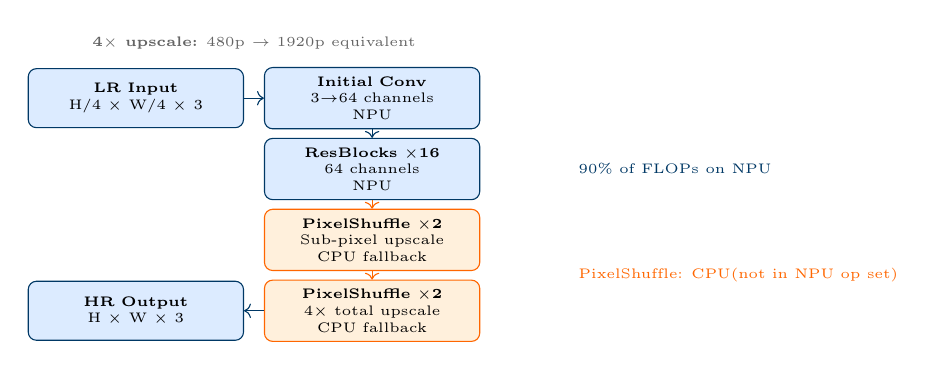
\begin{tikzpicture}[
  blk/.style={draw=NXPBlue,fill=LightBlue,rounded corners=3pt,
              minimum height=0.75cm,text width=2.5cm,align=center,font=\tiny},
  oblk/.style={draw=NXPOrange,fill=LightOrange,rounded corners=3pt,
               minimum height=0.75cm,text width=2.5cm,align=center,font=\tiny},
]
\node[blk] (lr) at (0,3.5) {\textbf{LR Input}\\H/4 $\times$ W/4 $\times$ 3};
\node[blk] (conv1) at (3.0,3.5) {\textbf{Initial Conv}\\3$\rightarrow$64 channels\\NPU};
\node[blk] (res) at (3.0,2.6) {\textbf{ResBlocks $\times$16}\\64 channels\\NPU};
\node[oblk] (ps1) at (3.0,1.7) {\textbf{PixelShuffle $\times$2}\\Sub-pixel upscale\\CPU fallback};
\node[oblk] (ps2) at (3.0,0.8) {\textbf{PixelShuffle $\times$2}\\4$\times$ total upscale\\CPU fallback};
\node[blk] (hr) at (0,0.8) {\textbf{HR Output}\\H $\times$ W $\times$ 3};
\draw[->,NXPBlue] (lr) -- (conv1);
\draw[->,NXPBlue] (conv1) -- (res);
\draw[->,NXPOrange] (res) -- (ps1);
\draw[->,NXPOrange] (ps1) -- (ps2);
\draw[->,NXPBlue] (ps2) -- (hr);
\node[font=\tiny,text=NXPBlue,anchor=west] at (5.5,2.6)
  {90\% of FLOPs on NPU};
\node[font=\tiny,text=NXPOrange,anchor=west] at (5.5,1.25)
  {PixelShuffle: CPU\\(not in NPU op set)};
\node[font=\tiny,text=NXPGray] at (1.5,4.2)
  {\textbf{4$\times$ upscale:} 480p $\rightarrow$ 1920p equivalent};
\end{tikzpicture}
\column{0.45\textwidth}
\footnotesize
\begin{block}{Fast-SRGAN Specs}
\begin{itemize}
  \item \textbf{168K parameters} --- extremely compact
  \item \textbf{PSNR}: $\sim$30 dB on Set5 benchmark
  \item Input: variable resolution (dynamic shape)
  \item Latency: $\sim$25ms on i.MX 8M Plus NPU
  \item Only 10\% of FLOPs fall back to CPU (PixelShuffle)
\end{itemize}
\end{block}
\begin{block}{SCI Low-Light}
\begin{itemize}
  \item \textbf{Dynamic shape}: any resolution
  \item 8 KB INT8 size --- extremely tiny
  \item \textbf{No resize needed}: full-res passthrough
  \item Improves face recognition +30\% in dark
\end{itemize}
\end{block}
\end{columns}
\end{frame}

\section{Audio Models}

\begin{frame}{Audio Models: KWS + ASR on NXP}
\begin{columns}
\column{0.50\textwidth}
\small
\begin{tabular}{lccl}
\toprule
\textbf{Model} & \textbf{Score} & \textbf{Platform} & \textbf{Task}\\
\midrule
microspeech\_lstm & 82\% & RT1170 & 4-word KWS\\
ds\_cnn & 94.0\% & i.MX 93 & 35-word KWS\\
wav2letter & WER 7.2\% & i.MX 8M Plus & Full ASR\\
anomaly\_ae & 93.0\% AUC & i.MX 93 & MIMII anomaly\\
\bottomrule
\end{tabular}
\vspace{0.4cm}
\begin{block}{wav2letter: Edge ASR}
\footnotesize
\begin{itemize}
  \item \textbf{Full sentence ASR} on edge device
  \item Input: (1, 296, 39) MFCC features
  \item CTC decoder on CPU (Beam search)
  \item Latency: $\sim$150ms / utterance
  \item \textbf{No cloud required} --- fully on-device
\end{itemize}
\end{block}
\column{0.47\textwidth}
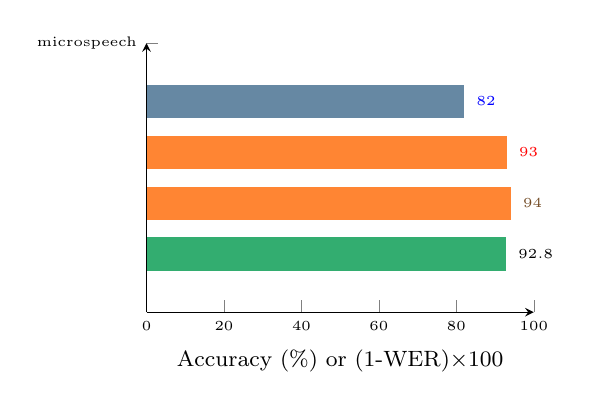
\begin{tikzpicture}
\begin{axis}[
  xbar,
  width=6.5cm,height=5.0cm,
  bar width=12pt,
  xlabel={\footnotesize Accuracy (\%) or (1-WER)$\times$100},
  ytick=data,
  yticklabels={microspeech,anomaly\_ae,ds\_cnn,wav2letter},
  yticklabel style={font=\tiny},
  xticklabel style={font=\tiny},
  xmin=0,xmax=100,
  nodes near coords,nodes near coords style={font=\tiny,xshift=1pt},
  axis lines=left,tick align=inside,
]
\addplot+[xbar,fill=NXPBlue!60,draw=none] coordinates {(82,3)};
\addplot+[xbar,fill=NXPOrange!80,draw=none] coordinates {(93.0,2)};
\addplot+[xbar,fill=NXPOrange!80,draw=none] coordinates {(94.0,1)};
\addplot+[xbar,fill=NXPGreen!80,draw=none] coordinates {(92.8,0)};
\end{axis}
\end{tikzpicture}
\end{columns}
\end{frame}

\section{Why Model Zoo Fits NXP Hardware}

\begin{frame}{TFLite Per-Channel INT8: Better Fit than Per-Tensor}
\begin{columns}
\column{0.52\textwidth}
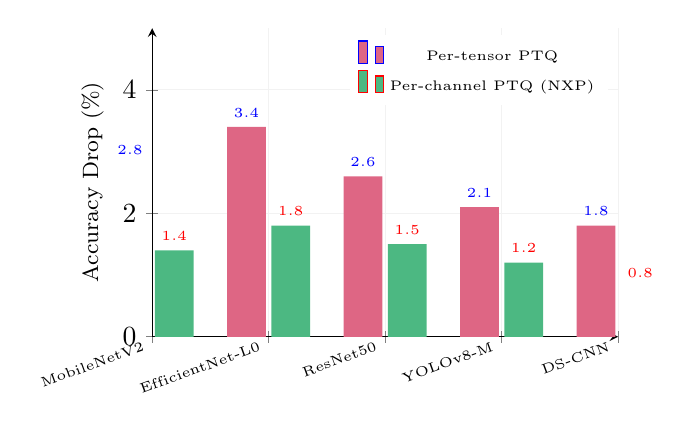
\begin{tikzpicture}
\begin{axis}[
  ybar,
  width=7.5cm,height=5.5cm,
  bar width=14pt,
  ylabel={\footnotesize Accuracy Drop (\%)},
  xtick=data,
  xticklabels={MobileNetV2,EfficientNet-L0,ResNet50,YOLOv8-M,DS-CNN},
  xticklabel style={font=\tiny,rotate=20,anchor=east},
  ymin=0,ymax=5,
  grid=major,grid style={gray!10},
  axis lines=left,
  legend style={font=\tiny,at={(0.98,0.98)},anchor=north east,draw=none},
  nodes near coords,nodes near coords style={font=\tiny},
]
\addplot+[fill=AccentRed!60,draw=none]
  coordinates {(0,2.8)(1,3.4)(2,2.6)(3,2.1)(4,1.8)};
\addlegendentry{Per-tensor PTQ}
\addplot+[fill=NXPGreen!70,draw=none]
  coordinates {(0,1.4)(1,1.8)(2,1.5)(3,1.2)(4,0.8)};
\addlegendentry{Per-channel PTQ (NXP)}
\end{axis}
\end{tikzpicture}
\column{0.45\textwidth}
\footnotesize
\begin{block}{Why Per-Channel is Better}
Per-channel quantization assigns one scale factor per output channel of each Conv2D layer (vs.\ one global scale for per-tensor). For models with large weight variance across channels (ResNet, EfficientNet), per-channel reduces accuracy loss by up to 2$\times$.
\end{block}
\begin{alertblock}{NXP Model Zoo Policy}
All models compiled with \texttt{TFLiteConverter.optimizations = [DEFAULT]} + \texttt{representative\_dataset}: 100--1000 calibration samples. Always per-channel INT8.
\end{alertblock}
\end{columns}
\end{frame}

\begin{frame}{Memory Budget: Model Fit per Platform}
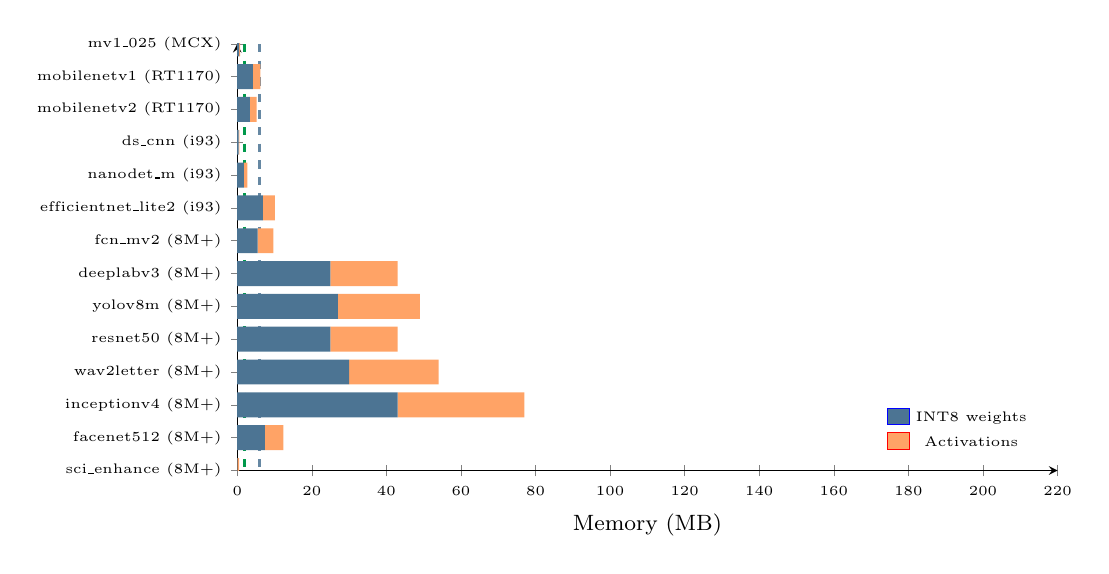
\begin{tikzpicture}
\begin{axis}[
  xbar stacked,
  width=12cm,height=7cm,
  bar width=9pt,
  xlabel={\footnotesize Memory (MB)},
  ytick=data,
  yticklabels={
    mv1\_025 (MCX),
    mobilenetv1 (RT1170),
    mobilenetv2 (RT1170),
    ds\_cnn (i93),
    nanodet\_m (i93),
    efficientnet\_lite2 (i93),
    fcn\_mv2 (8M+),
    deeplabv3 (8M+),
    yolov8m (8M+),
    resnet50 (8M+),
    wav2letter (8M+),
    inceptionv4 (8M+),
    facenet512 (8M+),
    sci\_enhance (8M+)
  },
  yticklabel style={font=\tiny},
  xticklabel style={font=\tiny},
  xlabel style={font=\tiny},
  legend style={font=\tiny,at={(0.98,0.02)},anchor=south east,draw=none},
  xmin=0,xmax=220,
  tick align=inside,axis lines=left,
]
\addplot+[xbar,fill=NXPBlue!70,draw=none]
  coordinates {(0.5,13)(4.2,12)(3.4,11)(0.4,10)(1.8,9)(6.9,8)
               (5.5,7)(25,6)(27,5)(25,4)(30,3)(43,2)(7.4,1)(0.01,0)};
\addplot+[xbar,fill=NXPOrange!60,draw=none]
  coordinates {(0.3,13)(2.0,12)(1.8,11)(0.2,10)(0.9,9)(3.2,8)
               (4.2,7)(18,6)(22,5)(18,4)(24,3)(34,2)(5.0,1)(0.5,0)};
\addlegendentry{INT8 weights}
\addlegendentry{Activations}
\draw[dashed,NXPGreen,line width=1pt] (axis cs:2,13.5) -- (axis cs:2,-0.5)
  node[below,font=\tiny,text=NXPGreen]{MCX 512KB};
\draw[dashed,NXPBlue!60,line width=1pt] (axis cs:6,13.5) -- (axis cs:6,-0.5)
  node[below,font=\tiny,text=NXPBlue!60]{RT1170 2MB};
\end{axis}
\end{tikzpicture}
\end{frame}

\begin{frame}{NPU Operator Coverage: Model-by-Model}
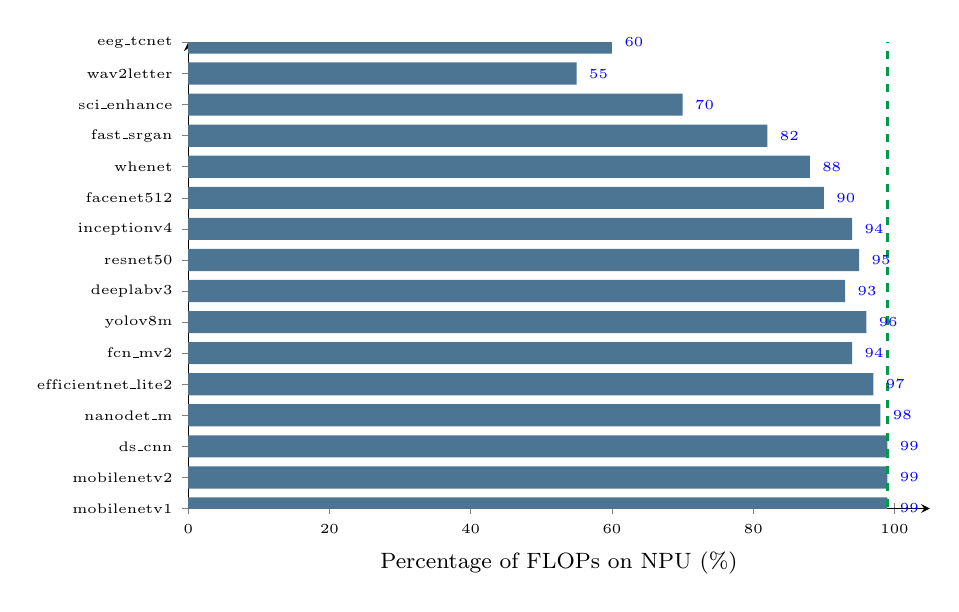
\begin{tikzpicture}
\begin{axis}[
  xbar,
  width=11cm,height=7.5cm,
  bar width=8pt,
  xlabel={\footnotesize Percentage of FLOPs on NPU (\%)},
  ytick=data,
  yticklabels={
    eeg\_tcnet,wav2letter,sci\_enhance,fast\_srgan,
    whenet,facenet512,inceptionv4,resnet50,deeplabv3,
    yolov8m,fcn\_mv2,efficientnet\_lite2,nanodet\_m,
    ds\_cnn,mobilenetv2,mobilenetv1
  },
  yticklabel style={font=\tiny},
  xticklabel style={font=\tiny},
  xmin=0,xmax=105,
  tick align=inside,axis lines=left,
  nodes near coords,nodes near coords style={font=\tiny,xshift=1pt},
]
\addplot+[xbar,fill=NXPBlue!70,draw=none] coordinates {
  (60,15)(55,14)(70,13)(82,12)
  (88,11)(90,10)(94,9)(95,8)(93,7)
  (96,6)(94,5)(97,4)(98,3)
  (99,2)(99,1)(99,0)
};
\draw[dashed,NXPGreen,line width=1pt] (axis cs:99,-0.5) -- (axis cs:99,15.5)
  node[above,font=\tiny,text=NXPGreen]{full NPU};
\end{axis}
\end{tikzpicture}
\end{frame}

\section{Performance Benchmarks}

\begin{frame}{Inference Latency: i.MX 8M Plus vs.\ i.MX 93}
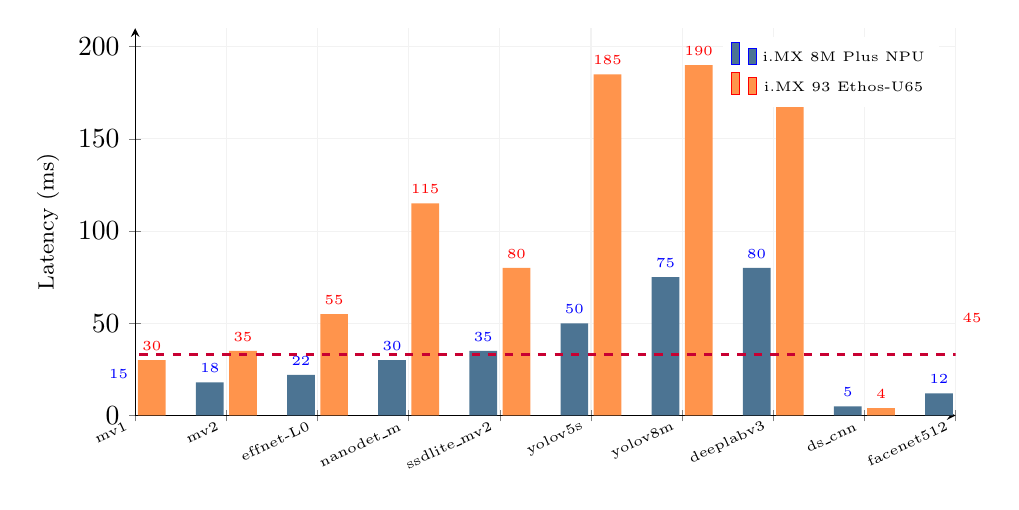
\begin{tikzpicture}
\begin{axis}[
  ybar,
  width=12cm,height=6.5cm,
  bar width=10pt,
  ylabel={\footnotesize Latency (ms)},
  xtick=data,
  xticklabels={mv1,mv2,effnet-L0,nanodet\_m,ssdlite\_mv2,yolov5s,yolov8m,deeplabv3,ds\_cnn,facenet512},
  xticklabel style={font=\tiny,rotate=25,anchor=east},
  ymin=0,ymax=210,
  grid=major,grid style={gray!10},
  axis lines=left,
  legend style={font=\tiny,at={(0.98,0.98)},anchor=north east,draw=none},
  nodes near coords,nodes near coords style={font=\tiny},
]
\addplot+[fill=NXPBlue!70,draw=none]
  coordinates {(0,15)(1,18)(2,22)(3,30)(4,35)(5,50)(6,75)(7,80)(8,5)(9,12)};
\addlegendentry{i.MX 8M Plus NPU}
\addplot+[fill=NXPOrange!70,draw=none]
  coordinates {(0,30)(1,35)(2,55)(3,115)(4,80)(5,185)(6,190)(7,185)(8,4)(9,45)};
\addlegendentry{i.MX 93 Ethos-U65}
\draw[dashed,AccentRed,line width=1pt] (axis cs:-0.5,33) -- (axis cs:9.5,33)
  node[right,font=\tiny,text=AccentRed]{33ms = 30 FPS};
\end{axis}
\end{tikzpicture}
\end{frame}

\begin{frame}{Power Efficiency: eIQ Platforms vs.\ Competitors}
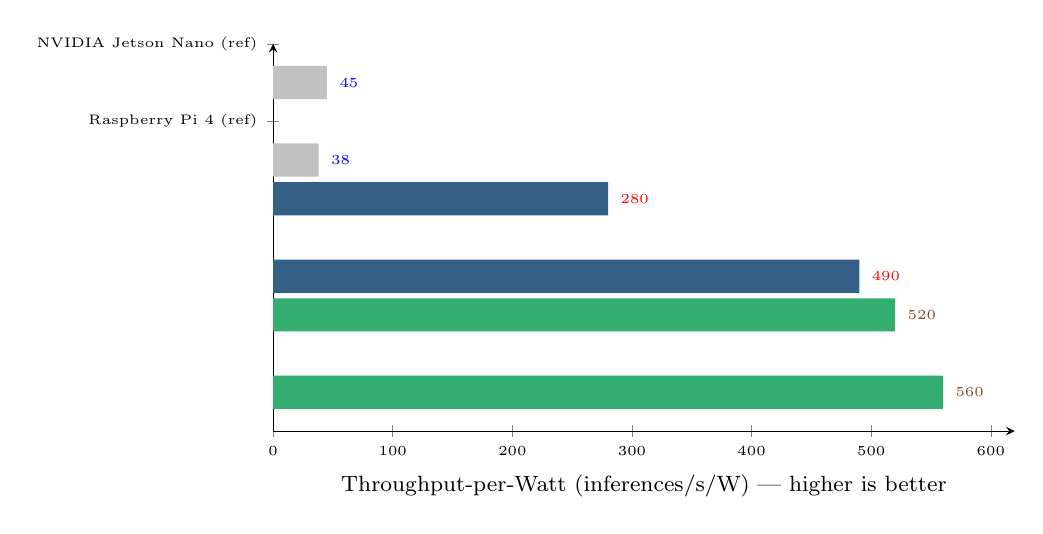
\begin{tikzpicture}
\begin{axis}[
  xbar,
  width=11cm,height=6.5cm,
  bar width=12pt,
  xlabel={\footnotesize Throughput-per-Watt (inferences/s/W) --- higher is better},
  ytick=data,
  yticklabels={
    NVIDIA Jetson Nano (ref),
    Raspberry Pi 4 (ref),
    NXP i.MX 8M Plus (MobileNetV2),
    NXP i.MX 93 (MobileNetV2 Ethos),
    NXP RT1170 (microspeech),
    NXP MCX N947 (mv1\_025)
  },
  yticklabel style={font=\tiny},
  xticklabel style={font=\tiny},
  xmin=0,xmax=620,
  tick align=inside,axis lines=left,
  nodes near coords,nodes near coords style={font=\tiny,xshift=1pt},
]
\addplot+[xbar,fill=NXPGray!40,draw=none] coordinates {(45,5)(38,4)};
\addplot+[xbar,fill=NXPBlue!80,draw=none] coordinates {(280,3)(490,2)};
\addplot+[xbar,fill=NXPGreen!80,draw=none] coordinates {(520,1)(560,0)};
\end{axis}
\end{tikzpicture}
\end{frame}

\section{Multi-Model Pipelines}

\begin{frame}{NXP Driver Monitoring System (DMS) Pipeline}
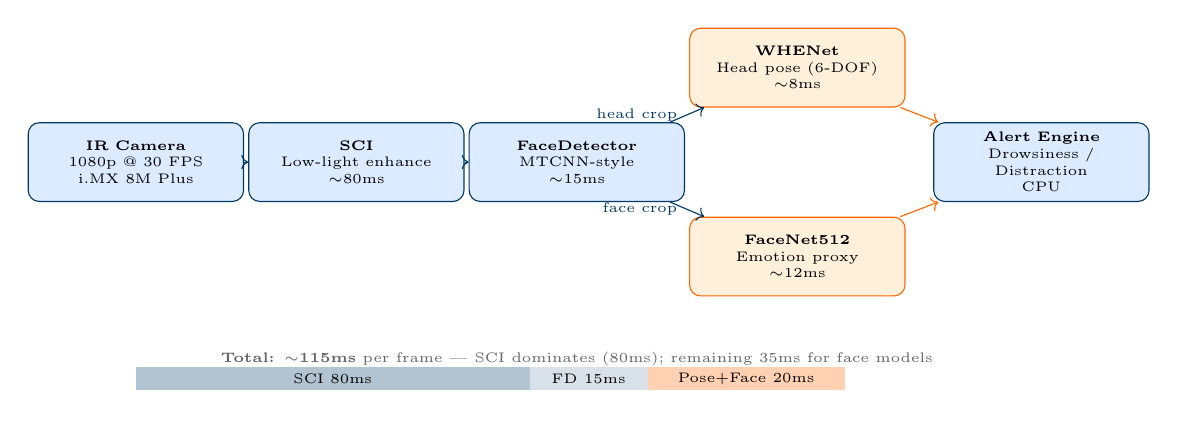
\begin{tikzpicture}[
  box/.style={draw=NXPBlue,fill=LightBlue,rounded corners=4pt,
              minimum height=1.0cm,text width=2.5cm,align=center,font=\tiny},
  obox/.style={draw=NXPOrange,fill=LightOrange,rounded corners=4pt,
               minimum height=1.0cm,text width=2.5cm,align=center,font=\tiny},
]
\node[box] (cam) at (0,2.0) {\textbf{IR Camera}\\1080p @ 30 FPS\\i.MX 8M Plus};
\node[box] (sci) at (2.8,2.0) {\textbf{SCI}\\Low-light enhance\\$\sim$80ms};
\node[box] (fd) at (5.6,2.0) {\textbf{FaceDetector}\\MTCNN-style\\$\sim$15ms};
\node[obox] (whe) at (8.4,3.2) {\textbf{WHENet}\\Head pose (6-DOF)\\$\sim$8ms};
\node[obox] (fn) at (8.4,0.8) {\textbf{FaceNet512}\\Emotion proxy\\$\sim$12ms};
\node[box] (alert) at (11.5,2.0) {\textbf{Alert Engine}\\Drowsiness /\\Distraction\\CPU};
\draw[->,NXPBlue] (cam) -- (sci);
\draw[->,NXPBlue] (sci) -- (fd);
\draw[->,NXPBlue] (fd) -- (whe) node[midway,left,font=\tiny]{head crop};
\draw[->,NXPBlue] (fd) -- (fn) node[midway,left,font=\tiny]{face crop};
\draw[->,NXPOrange] (whe) -- (alert);
\draw[->,NXPOrange] (fn) -- (alert);
\node[font=\tiny,text=NXPGray] at (5.6,-0.5)
  {\textbf{Total: $\sim$115ms} per frame --- SCI dominates (80ms); remaining 35ms for face models};
\draw[fill=NXPBlue!30,draw=none] (0,-0.9) rectangle (5.0,-0.6)
  node[midway,font=\tiny]{SCI 80ms};
\draw[fill=NXPBlue!15,draw=none] (5.0,-0.9) rectangle (6.5,-0.6)
  node[midway,font=\tiny]{FD 15ms};
\draw[fill=NXPOrange!30,draw=none] (6.5,-0.9) rectangle (9.0,-0.6)
  node[midway,font=\tiny]{Pose+Face 20ms};
\end{tikzpicture}
\end{frame}

\begin{frame}{NXP Low-Light Face Recognition Pipeline}
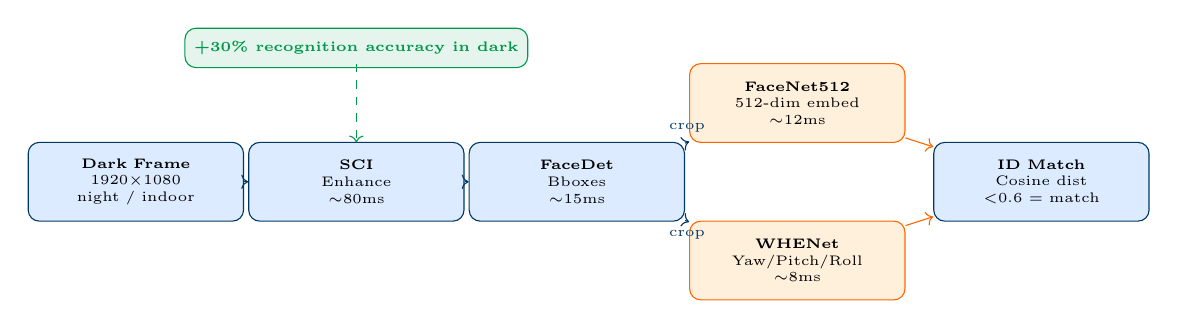
\begin{tikzpicture}[
  box/.style={draw=NXPBlue,fill=LightBlue,rounded corners=4pt,
              minimum height=1.0cm,text width=2.5cm,align=center,font=\tiny},
  obox/.style={draw=NXPOrange,fill=LightOrange,rounded corners=4pt,
               minimum height=1.0cm,text width=2.5cm,align=center,font=\tiny},
]
\node[box] (frame) at (0,1.5) {\textbf{Dark Frame}\\1920$\times$1080\\night / indoor};
\node[box] (sci) at (2.8,1.5) {\textbf{SCI}\\Enhance\\$\sim$80ms};
\node[box] (fdet) at (5.6,1.5) {\textbf{FaceDet}\\Bboxes\\$\sim$15ms};
\node[obox] (fn) at (8.4,2.5) {\textbf{FaceNet512}\\512-dim embed\\$\sim$12ms};
\node[obox] (whe) at (8.4,0.5) {\textbf{WHENet}\\Yaw/Pitch/Roll\\$\sim$8ms};
\node[box] (id) at (11.5,1.5) {\textbf{ID Match}\\Cosine dist\\$<$0.6 = match};
\draw[->,NXPBlue] (frame) -- (sci);
\draw[->,NXPBlue] (sci) -- (fdet);
\draw[->,NXPBlue] (fdet) -- (fn) node[midway,font=\tiny,above]{crop};
\draw[->,NXPBlue] (fdet) -- (whe) node[midway,font=\tiny,below]{crop};
\draw[->,NXPOrange] (fn) -- (id);
\draw[->,NXPOrange] (whe) -- (id);
\node[draw=NXPGreen,fill=NXPGreen!10,rounded corners,
      font=\tiny\bfseries,text=NXPGreen,
      minimum width=3.5cm,minimum height=0.5cm] at (2.8,3.2)
  {+30\% recognition accuracy in dark};
\draw[->,dashed,NXPGreen] (2.8,3.0) -- (2.8,2.0);
\end{tikzpicture}
\end{frame}

\section{Development Ecosystem}

\begin{frame}{NXP eIQ Development Ecosystem}
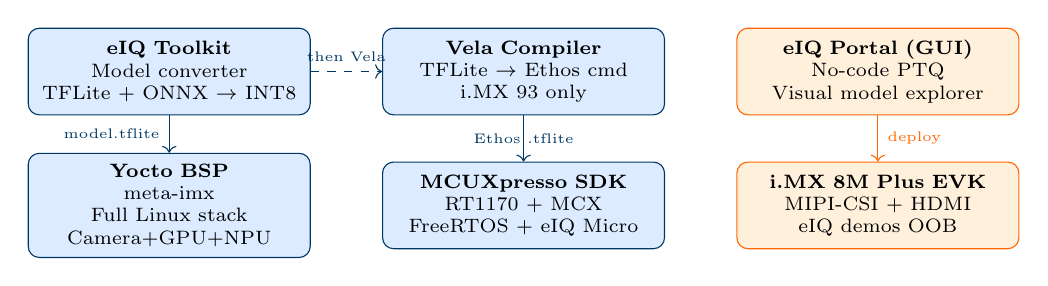
\begin{tikzpicture}[
  tool/.style={draw=NXPBlue,fill=LightBlue,rounded corners=4pt,
               minimum width=3.5cm,minimum height=1.1cm,
               text width=3.3cm,align=center,font=\scriptsize,inner sep=4pt},
  otool/.style={draw=NXPOrange,fill=LightOrange,rounded corners=4pt,
                minimum width=3.5cm,minimum height=1.1cm,
                text width=3.3cm,align=center,font=\scriptsize,inner sep=4pt},
]
\node[tool] (eiqtk) at (0,3.5) {\textbf{eIQ Toolkit}\\Model converter\\TFLite + ONNX $\rightarrow$ INT8};
\node[tool] (vela) at (4.5,3.5) {\textbf{Vela Compiler}\\TFLite $\rightarrow$ Ethos cmd\\i.MX 93 only};
\node[otool] (eiqportal) at (9.0,3.5) {\textbf{eIQ Portal (GUI)}\\No-code PTQ\\Visual model explorer};
\node[tool] (yocto) at (0,1.8) {\textbf{Yocto BSP}\\meta-imx\\Full Linux stack\\Camera+GPU+NPU};
\node[tool] (mcusdk) at (4.5,1.8) {\textbf{MCUXpresso SDK}\\RT1170 + MCX\\FreeRTOS + eIQ Micro};
\node[otool] (evk) at (9.0,1.8) {\textbf{i.MX 8M Plus EVK}\\MIPI-CSI + HDMI\\eIQ demos OOB};
\draw[->,NXPBlue] (eiqtk) -- (yocto)
  node[midway,left,font=\tiny]{model.tflite};
\draw[->,NXPBlue] (vela) -- (mcusdk)
  node[midway,font=\tiny]{Ethos .tflite};
\draw[->,NXPOrange] (eiqportal) -- (evk)
  node[midway,right,font=\tiny]{deploy};
\draw[->,NXPBlue,dashed] (eiqtk) -- (vela)
  node[midway,above,font=\tiny]{then Vela};
\end{tikzpicture}
\end{frame}

\begin{frame}{MLOps Pipeline for NXP eIQ}
\small
\begin{tabular}{llll}
\toprule
\textbf{Stage} & \textbf{Tool} & \textbf{Artifact} & \textbf{Gate}\\
\midrule
Experiment tracking & MLflow & run metrics, PTQ params & ---\\
PTQ + Vela compile & recipe.sh + Optuna HPO & .tflite + .tosa & Acc/PSNR/WER gate\\
Model registry & MLflow Registry & Staging $\rightarrow$ Production & Threshold per task\\
Orchestration & Prefect 2 flows & Docker recipe DAG & Retries on failure\\
Drift detection & Evidently + PSNR drift & Acc + PSNR drift & $>$5\% drift $\rightarrow$ alert\\
CI/CD & GitHub Actions & 6-job pipeline & All gates pass\\
Infrastructure & AWS CDK v2 (Fargate) & S3+ECR+ECS+CW & CloudWatch alarms\\
\bottomrule
\end{tabular}
\vspace{0.3cm}
\begin{block}{Optuna HPO Parameters}
\footnotesize Tunes: \texttt{num\_calib\_steps} (100--2000), \texttt{dataset\_size} (100--1000), \texttt{per\_channel} (True/False), \texttt{vela\_memory\_config} (sram-only / sram+flash). Objective: maximize accuracy/PSNR within latency budget.
\end{block}
\end{frame}

\begin{frame}{Summary: NXP eIQ at a Glance}
\begin{columns}
\column{0.55\textwidth}
\small
\begin{tabular}{lcc}
\toprule
\textbf{Dimension} & \textbf{Score} & \textbf{Notes}\\
\midrule
Task diversity & $\bigstar\bigstar\bigstar\bigstar\bigstar$ & 11 categories, 29 models\\
Unique capabilities & $\bigstar\bigstar\bigstar\bigstar\bigstar$ & SR, BCI, face recog\\
Classification acc. & $\bigstar\bigstar\bigstar\bigstar$ & 78.2\% InceptionV4\\
Detection acc. & $\bigstar\bigstar\bigstar\bigstar$ & 53.5\% YOLOv8-M\\
Power efficiency & $\bigstar\bigstar\bigstar$ & 0.5--8W range\\
Quantization ease & $\bigstar\bigstar\bigstar\bigstar\bigstar$ & recipe.sh Docker, simple\\
NPU coverage & $\bigstar\bigstar\bigstar\bigstar$ & $>$90\% for CNNs\\
Vela (Ethos-U65) & $\bigstar\bigstar\bigstar\bigstar$ & 2--4$\times$ speedup on i93\\
Dev ecosystem & $\bigstar\bigstar\bigstar\bigstar\bigstar$ & eIQ Portal + Yocto SDK\\
Audio support & $\bigstar\bigstar\bigstar\bigstar$ & KWS + full ASR\\
\bottomrule
\end{tabular}
\column{0.42\textwidth}
\begin{block}{Key Differentiators}
\begin{itemize}
  \item \textbf{Broadest task coverage}: 11 categories
  \item \textbf{Only zoo with}: SR, low-light enhance, face recognition, BCI/EEG
  \item \textbf{TFLite standard}: simplest deployment path
  \item \textbf{Vela + Ethos-U65}: 2--4$\times$ speedup on i.MX 93
  \item \textbf{recipe.sh}: reproducible Docker PTQ in minutes
\end{itemize}
\end{block}
\begin{alertblock}{Best Fit When\ldots}
\footnotesize Widest task coverage needed, or specifically face recognition, super-resolution, ASR, or BCI. Also best when Linux Yocto deployment and TFLite familiarity matter.
\end{alertblock}
\end{columns}
\end{frame}

\end{document}
